%%%%%%%%%%%%%%%%%%%%%%%%%%%%%%%%%%%%%%%%%%%%%%%%%%%%%%%%%%%%%%%%%%%%%%%%%%%
\documentclass{article}
%%%%%%%%%%%%%%%%%%%%%%%%%%%%%%%%%%%%%%%%%%%%%%%%%%%%%%%%%%%%%%%%%%%%%%%%%%%

\usepackage{amssymb}
\usepackage{amsmath}
\usepackage{amsfonts}
\usepackage{amsthm}
\usepackage{graphicx}
\usepackage{tikz}
%%%%%%%%%%%%%%%%%%%%%%%%%%%%%%%%%%%%%%%%%%%%%%%%%%%%%%%%%%%%%%%%%%%%%%%
% This file contains every macro I've used in my master's thesis.     %
%                                                                     %
% Macros that are used for specific kinds of logics and/or proofs are %
% organised by topic. More general macros appear at the top, such as  %
% typesetting conventions and higher-order functions. The aim is to   %
% end up with a macro file I can use for research in the future with  %
% a consistent style convention, and also to make it easy to restyle  %
% my thesis should the need arise.                                    %
%                                                                     %
% The convention is that commands that are intended to be written     %
% inline, such as logical connectives, get lowercase names. Commands  %
% that refer to a particular mathematical object, such as a set of    %
% atoms, get uppercase names.                                         %
%%%%%%%%%%%%%%%%%%%%%%%%%%%%%%%%%%%%%%%%%%%%%%%%%%%%%%%%%%%%%%%%%%%%%%%

%%%%%%%%%%%%%%%%%%%%%%%%%%%%%%%%%%%%%%%%%%%%%%%%%%
% Typesetting and/or Stylistic Conventions       %
%%%%%%%%%%%%%%%%%%%%%%%%%%%%%%%%%%%%%%%%%%%%%%%%%%

% Page geometry and styling.
\setlength{\parskip}{0.5em}
\setlength{\parindent}{0.5em}

% Mathematics environments.
\newtheorem{lemma}{Lemma}
\newtheorem{theorem}{Theorem}
\newtheorem{definition}{Definition}
\newtheorem{example}{Example}
\newtheorem{corollary}{Corollary}

% Algorithm environments.
% \SetKwInput{KwData}{Input}
% \SetKwInput{KwResult}{Output}

% Font styles for various things.
\newcommand{\textprop}[1]{\textsc{#1}} % entailment/satisfaction properties
\newcommand{\textlog}[1]{\textsc{#1}} % names of logics
\newcommand{\textpred}[1]{\textsf{\upshape#1}} % predicates in examples
\newcommand{\textop}[1]{\textrm{#1}} % mathematical operators
\newcommand{\textcomp}[1]{\textsc{#1}} % complexity classes
\newcommand{\textalgo}[1]{\textsf{#1}} % algorithm names

% Aliases and shorthands for the most common things.
\newcommand{\tp}{\textpred}

%%%%%%%%%%%%%%%%%%%%%%%%%%%%%%%%%%%%%%%%%%%%%%%%%%
% Global Mathematical Objects                    %
%%%%%%%%%%%%%%%%%%%%%%%%%%%%%%%%%%%%%%%%%%%%%%%%%%

% Abbreviated names for various logics.
\newcommand{\Klm}{\textlog{Klm}} % propositional KLM
\newcommand{\Alc}{\textlog{Alc}} % description logic ALC
\newcommand{\Ptl}{\textlog{Ptl}} % propositional typicality logic
\newcommand{\Sql}{\textlog{Sql}} % SQL database query language

% Complexity classes.
\newcommand{\Exptime}{\textcomp{Exptime}} % EXPTIME
\newcommand{\NpComplete}{\textcomp{NP-Complete}} % EXPTIME

% Languages, signatures and sets of symbols.
\newcommand{\Lang}{\ensuremath{\mathcal{L}}} % general language
\newcommand{\Univ}{\mathcal{U}} % set of possible worlds

% Entailment relations and their global properties.
\newcommand{\entails}{\models} % classical entailment
\newcommand{\nentails}{\not\entails}
\newcommand{\dentails}{\mid\hskip-0.40ex\approx} % defeasible entailment
\newcommand{\ndentails}{\not\mid\hskip-0.40ex\approx}
\newcommand{\genentails}{\entails_?} % placeholder entailment relation
\newcommand{\entincl}{\textprop{(Incl)}}
\newcommand{\entidem}{\textprop{(Idem)}}
\newcommand{\entcumu}{\textprop{(Cumu)}}
\newcommand{\entmono}{\textprop{(Mono)}}
\newcommand{\entsmp}{\textprop{(Smp)}}

% Abbreviations for KLM rationality properties
\newcommand{\klmlle}{\textprop{(Lle)}} % left logical equivalence
\newcommand{\klmrw}{\textprop{(Rw)}} % right weakening
\newcommand{\klmrefl}{\textprop{(Refl)}} % reflexivity
\newcommand{\klmand}{\textprop{(And)}} % conjunction in the conclusion
\newcommand{\klmor}{\textprop{(Or)}} % disjunction in the premise
\newcommand{\klmcut}{\textprop{(Cut)}} % cut rule
\newcommand{\klmcm}{\textprop{(Cm)}} % cautious monotonicity
\newcommand{\klmrm}{\textprop{(Rm)}} % rational monotonicity
\newcommand{\klmcons}{\textprop{(Cons)}} % consistency
\newcommand{\klmsc}{\textprop{(Sc)}} % supraclassicality
\newcommand{\klmmon}{\textprop{(Mon)}} % monotonicity
\newcommand{\klmtrans}{\textprop{(Trans)}} % transitivity

% Standard mathematical objects, like numbers.
\newcommand{\Nat}{\mathbb{N}} % naturals
\newcommand{\NatInf}{\mathbb{N}^\infty} % naturals with top element
\newcommand{\Int}{\mathbb{Z}} % integers

% Satisfaction and satisfaction sets.
\newcommand{\SatS}{\mathcal{S}} % satisfaction set
\newcommand{\sat}{\Vdash} % satisfaction relation
\newcommand{\nsat}{\not\sat}

% Ranking functions.
\newcommand{\rk}{\textop{rk}} % ranking function

% Knowledge bases and various functions of them.
\newcommand{\KB}{\ensuremath{\mathcal{K}}} % knowledge base
\newcommand{\Mod}[1]{\textop{Mod}(#1)} % models of a KB

%%%%%%%%%%%%%%%%%%%%%%%%%%%%%%%%%%%%%%%%%%%%%%%%%%
% First-Order Logic                              %
%%%%%%%%%%%%%%%%%%%%%%%%%%%%%%%%%%%%%%%%%%%%%%%%%%

% Languages, symbols and signatures.
\newcommand{\LangFol}{\Lang} % first-order language (as in set of all wffs)
\newcommand{\FolLang}{\Sigma} % first-order language (as in signature)
\newcommand{\FolLangVar}{\textsc{var}} % set of variable symbols
\newcommand{\FolLangPred}{\textsc{pred}} % set of predicate symbols
\newcommand{\FolLangConst}{\textsc{const}} % set of constant symbols
\newcommand{\FolLangFunc}{\textsc{func}} % set of function symbols
\newcommand{\FolLangTerms}{\mathcal{T}} % set of terms
\newcommand{\folLangArity}[1]{\mathfrak{ar}(#1)} % arity of predicate symbol

% Standard semantics
\newcommand{\FolI}{\mathcal{I}} % first-order structure
\newcommand{\FolISet}{\mathscr{I}} % set of all first-order structures
\newcommand{\FolDom}[1]{\Delta^{#1}} % first-order domain
\newcommand{\FolFun}[2]{{#2}^{#1}} % first-order interpretation function
\newcommand{\FolVal}{\upsilon} % first-order valuation function

% Herbrand semantics.
\newcommand{\HerbU}{\mathbb U} % herbrand universe, i.e. set of terms
\newcommand{\HerbB}{\mathbb B} % herbrand base, i.e. set of ground atoms
\newcommand{\HerbI}{\mathcal{H}} % herbrand interpretation
\newcommand{\HerbISet}{\mathbb{H}} % set of all herbrand interpretations

%%%%%%%%%%%%%%%%%%%%%%%%%%%%%%%%%%%%%%%%%%%%%%%%%%
% Propositional KLM                              %
%%%%%%%%%%%%%%%%%%%%%%%%%%%%%%%%%%%%%%%%%%%%%%%%%%

% Propositional KLM versions of languages, signatures etc.
\newcommand{\LangKLM}{\Lang^{\twiddle}} % defeasible propositional formulas
\newcommand{\Prp}{\ensuremath{\mathcal{P}}} % propositional atoms
\newcommand{\Th}[1]{\mathrm{Th}(#1)} % deductive closure

% Simplified propositional logic connectives.
\newcommand{\limp}{\rightarrow} % logical implication
\newcommand{\liff}{\leftrightarrow} % biconditional
\newcommand{\lexor}{\oplus} % exclusive or

% The twiddle symbol for defeasible consequence relations.
\newcommand{\twiddle}{\mathrel|\joinrel\sim}
\newcommand{\ntwiddle}{\not\twiddle}

% Various forms of defeasible entailment.
\newcommand{\prefentails}{\entails_{\PrefI}} % preferential entailment
\newcommand{\rankentails}{\entails_{\RankI}} % ranked entailment
\newcommand{\rcentails}{\dentails_{RC}} % rational closure entailment

% Preferential and ranked interpretations.
\newcommand{\PrefI}{\ensuremath{\mathcal{P}}} % preferential interpretation
\newcommand{\ModI}{\ensuremath{\mathcal{M}}} % modular interpretation
\newcommand{\RankI}{\ensuremath{\mathcal{R}}} % ranked interpretation
\newcommand{\rankleq}{\leq_G} % typicality ordering on ranked interpretations

% Possible worlds and such for satisfaction.
\newcommand{\Poss}[1]{\widehat{#1}} % set of possible worlds for a formula
\newcommand{\Cons}[1]{\Univ^{#1}} % set of possible worlds for an interpretation

% Materialisation and exceptionality for computing rational closure.
\newcommand{\Mat}[1]{\ensuremath{{#1}^{\limp}}}

% Algorithms for computing rational closure.
\newcommand{\BaseRank}[1]{\textop{br}({#1})} % baserank for formulas
\newcommand{\BaseRankAlg}{\textalgo{BaseRank}} % baserank algorithm
\newcommand{\RationalClosureAlg}{\textalgo{RationalClosure}} % rc algorithm

%%%%%%%%%%%%%%%%%%%%%%%%%%%%%%%%%%%%%%%%%%%%%%%%%%
% Defeasible Description Logics                  %
%%%%%%%%%%%%%%%%%%%%%%%%%%%%%%%%%%%%%%%%%%%%%%%%%%

% Languages, signatures and sets of symbols.
\newcommand{\LangALC}{\Lang^\Alc}
\newcommand{\Concepts}{\ensuremath{\mathcal{C}}} % set of concept names
\newcommand{\Roles}{\ensuremath{\mathcal{R}}} % set of role names
\newcommand{\Individuals}{\ensuremath{\mathcal{I}}} % set of individual names
\newcommand{\ABox}{\ensuremath{\mathcal{A}}} % set of a-box statements
\newcommand{\TBox}{\ensuremath{\mathcal{T}}} % set of t-box statements
\newcommand{\DBox}{\ensuremath{\mathcal{D}}} % set of defeasible t-box statements
\newcommand{\LangALCTBox}{\LangALC_\TBox} % set of t-box statements
\newcommand{\LangALCDBox}{\LangALC_\DBox} % set of defeasible t-box statements
\newcommand{\LangALCABox}{\LangALC_\ABox} % set of t-box statements

% Connectives for description logics. 
\newcommand{\dlAnd}{\sqcap} % concept conjunction
\newcommand{\dlOr}{\sqcup} % concept disjunction
\newcommand{\dlNot}{\lnot} % concept negation
\newcommand{\dlEquiv}{\equiv} % concept conjunction
\newcommand{\dlForall}[2]{\forall {#1} . {#2}} % value restriction
\newcommand{\dlExists}[2]{\exists {#1} . {#2}} % existential restriction
\newcommand{\subs}{\sqsubseteq} % concept subsumption
\newcommand{\nsubs}{\not\subs}
\newcommand{\dsubs}{\:\raisebox{0.45ex}{\ensuremath{\sqsubset}}\hskip-1.7ex\raisebox{-0.6ex}{\scalebox{0.9}{\ensuremath{\sim}}}\:} % defeasible subsumption
\newcommand{\ndsubs}{\not\hspace{-1.1mm}\dsubs}

% Interpretations and such.
\newcommand{\DlI}{\ensuremath{\mathcal{I}}} % dl interpretation
\newcommand{\DlFun}[2]{{#2}^{#1}} % dl interpretation function
\newcommand{\DlDom}[1]{\Delta^{#1}} % dl interpretation domain
\newcommand{\DlClassFun}[1]{\DlFun{\DlI}{#1}} % classical interpretation function
\newcommand{\DlClassDom}{\DlDom{\DlI}} % classical domain
\newcommand{\DlPrefFun}[1]{\DlFun{\PrefI}{#1}} % preferential interpretation function
\newcommand{\DlPrefDom}{\DlDom{\PrefI}} % preferential domain
\newcommand{\DlModFun}[1]{\DlFun{\ModI}{#1}} % modular interpretation function
\newcommand{\DlModDom}{\DlDom{\ModI}} % modular domain
\newcommand{\DlRankFun}[1]{\DlFun{\RankI}{#1}} % ranked interpretation function
\newcommand{\DlRankDom}{\DlDom{\RankI}} % ranked domain

% Big models, compatible models, and rankings of models.
\newcommand{\DlBigModel}[1]{\RankI(#1)} % big ranked model of a knowledge base
\newcommand{\DlCompatibleModels}[3]{\mathbb{R}^{#1,#2,#3}} % set of compatible ranked models
\newcommand{\dlrankleq}[1]{\leq_{#1}} % I-compatible ranking
\newcommand{\dlaboxleq}[1]{\leq^{A}_{#1}} % I-compatible A-Box ranking

%%%%%%%%%%%%%%%%%%%%%%%%%%%%%%%%%%%%%%%%%%%%%%%%%%
% Defeasible Datalog                             %
%%%%%%%%%%%%%%%%%%%%%%%%%%%%%%%%%%%%%%%%%%%%%%%%%%

% Classical datalog formulas.
\newcommand{\LangDlog}{\Lang} % classical datalog formulas
\newcommand{\LangDlogFacts}{\Lang_{f}} % classical datalog facts
\newcommand{\LangDlogRules}{\Lang_{\limp}} % classical datalog rules
\newcommand{\DlogLangPredEDB}{\FolLangPred_{E}} % EDB predicate symbols
\newcommand{\DlogLangPredIDB}{\FolLangPred_{I}} % IDB predicate symbols

% Defeasible datalog formulas.
\newcommand{\LangDDlog}{\Lang} % defeasible datalog formulas
\newcommand{\LangDDlogCompounds}{\Lang_{c}} % defeasible datalog compounds
\newcommand{\LangDDlogFacts}{\Lang_{f}} % classical datalog facts
\newcommand{\LangDDlogRules}{\Lang_{\limp}} % classical datalog rules
\newcommand{\LangDDlogDRules}{\Lang_{\dlimp}} % defeasible datalog rules

% Connectives for defeasible implication.
\newcommand{\dlimp}{\leadsto} % defeasible implication ~>
\newcommand{\ndlimp}{\,{\not \rightsquigarrow}\,}
\newcommand{\ldlimp}{\;\reflectbox{$\dlimp$}\;} % defeasible implication <~
\newcommand{\nldlimp}{\;\reflectbox{$\ndlimp$}\;}
\newcommand{\llimp}{\,:\!\!\!-\;} % classical implication :-

% Programs, databases and theories.
\newcommand{\DlogProg}{\mathcal{P}} % Datalog program
\newcommand{\DlogDat}{\mathcal{D}} % Datalog database
\newcommand{\DlogTheory}{\Gamma} % Datalog theory

% Substitutions.
\newcommand{\HerbSub}{\varphi} % substitution
\newcommand{\HerbSubId}{\varphi_\mathfrak{1}} % identity substitution

% Logical semantics and translations.
\newcommand{\DlogToFol}{\textop{Tr}} % datalog to FOL translation

% Enriched versions of things for typicality constants (TODO).
\newcommand{\herbS}{\mathcal{T}} % set of typical constants
\newcommand{\eherbB}{\herbB_\herbS} % enriched herbrand base
\newcommand{\eherbU}{\herbU_\herbS} % enriched herbrand universe
\newcommand{\eherbAll}{\herbAll_\herbS} % set of enriched herbrand ints.
\newcommand{\eherbI}{\mathcal{E}} % enriched herbrand int.


%%%%%%%%%%%%%%%%%%%%%%%%%%%%%%%%%%%%%%%%%%%%%%%%%%%%%%%%%%%%%%%%%%%%%%%%%%%
\begin{document}
%%%%%%%%%%%%%%%%%%%%%%%%%%%%%%%%%%%%%%%%%%%%%%%%%%%%%%%%%%%%%%%%%%%%%%%%%%%

\title{Territory and Conquest}
\author{Braden do Perez, Guy Paterson-Jones}

\maketitle

\begin{abstract}
  A study of a dynamical system on graphs that models territory control and conquest, loosely based on the board game \emph{Risk}. Every vertex is controlled by one of two players (black and white), and at each turn a vertex can change ownership based on influence from neighbouring vertices. Despite having somewhat simple rules, we describe a number of elusive conjectures about these dyamical systems that we are unable to prove. \cite{KrausEtAl1990}
\end{abstract}

%%%%%%%%%%%%%%%%%%%%%%%%%%%%%%%%%%%%%%%%%%%%%%%%%%%%%%%%%%%%%%%%%%%%%%%%%%%
\section{Introduction}
%%%%%%%%%%%%%%%%%%%%%%%%%%%%%%%%%%%%%%%%%%%%%%%%%%%%%%%%%%%%%%%%%%%%%%%%%%%

In the board game \emph{Risk}, the world consists of a number of territories, which are connected to each other by borders and sea routes. Each player controls one or more of these territories by placing armies on them, and each turn players can use these armies to wrest control of neighbouring territories from their opponents. In the standard rule set, a player wins the game when they either control every territory, or all of their opponents resign.

In these notes, we describe a simplified graph-theoretic model of a game of Risk. The idea is to model the state of the game at a particular point in time as a \emph{labelled graph}, where vertices represent territories, edges represent the connections between territories, and the label (or \emph{colour}) of a vertex represents the player that owns it. A game turn is modelled by an \emph{update function}, which changes the colours of the graph's vertices according to the colours of their neighbours. For instance, if a white vertex is surrounded by many black vertices, then the update function will change the colour of the white vertex to black. The following diagram should make the idea clear:

\begin{center}
  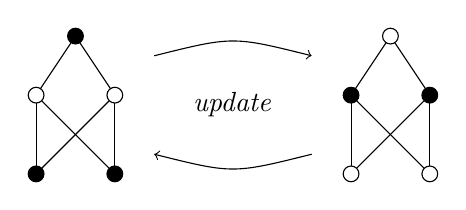
\begin{tikzpicture}
    % Leftmost graph:
    \draw (0,1) -- (0,0);
    \draw (1,1) -- (1,0);
    \draw (0,1) -- (1,0);
    \draw (1,1) -- (0,0);
    \draw (0.5,1.75) -- (0,1);
    \draw (0.5,1.75) -- (1,1);
    \filldraw[fill=black] (0.5,1.75) circle (0.1);
    \filldraw[fill=black] (0,0) circle (0.1);
    \filldraw[fill=white] (0,1) circle (0.1);
    \filldraw[fill=black] (1,0) circle (0.1);
    \filldraw[fill=white] (1,1) circle (0.1);

    % Rightmost graph:
    \draw (4,1) -- (4,0);
    \draw (5,1) -- (5,0);
    \draw (4,1) -- (5,0);
    \draw (5,1) -- (4,0);
    \draw (4.5,1.75) -- (4,1);
    \draw (4.5,1.75) -- (5,1);
    \filldraw[fill=white] (4.5,1.75) circle (0.1);
    \filldraw[fill=white] (4,0) circle (0.1);
    \filldraw[fill=black] (4,1) circle (0.1);
    \filldraw[fill=white] (5,0) circle (0.1);
    \filldraw[fill=black] (5,1) circle (0.1);

    % Update function arrows:
    \draw[->] (1.5,1.5) .. controls (2.5,1.75) .. (3.5,1.5);
    \draw[<-] (1.5,0.25) .. controls (2.5,0) .. (3.5,0.25);
    \draw (2.5,0.875) node {\emph{update}};
  \end{tikzpicture}
\end{center}

For simplicity, we will focus on the version of the model with two players, represented by the colours black and white. Nevertheless, the model hides a surprising amount of complexity. For instance, if one takes any finite black/white labelled graph and repeatedly applies the update function to it, one of two things eventually happens:

\begin{enumerate}
  \item The graph becomes monochromatic, i.e. one of the players wins.
  \item The graph settles into a periodic cycle, i.e. the same states keep occuring.
\end{enumerate}

The example we drew above is a periodic cycle of length $2$, since applying the update function repeatedly just alternates between the two graphs. In fact, \emph{every} case of a periodic cycle we've managed to come up with has length $2$! This leads us to conjecture that $2$ is the only possible length for a periodic cycle on a finite graph, but to date we have been unable to prove this.

%%%%%%%%%%%%%%%%%%%%%%%%%%%%%%%%%%%%%%%%%%%%%%%%%%%%%%%%%%%%%%%%%%%%%%%%%%%
\section{Choosing the Rules}
%%%%%%%%%%%%%%%%%%%%%%%%%%%%%%%%%%%%%%%%%%%%%%%%%%%%%%%%%%%%%%%%%%%%%%%%%%%

\newcommand{\selfDef}{\textsc{Sd}}
\newcommand{\nselfDef}{\neg \textsc{Sd}}
\newcommand{\tieNeu}{\textsc{Neu}}
\newcommand{\ntieNeu}{\neg \textsc{Neu}}

The main intuition we want to capture is that a vertex changes colour whenever its neighbourhood contains more \emph{enemies} than \emph{allies}. This raises (at least) two questions about the specifics of the update function:

\begin{enumerate}
  \item Does the vertex itself count as an allie? (``\emph{self-defence}'')
  \item What happens in the event of a tie? (``\emph{tie-breaking}'')
\end{enumerate}

Each of these questions leads to two obvious choices, for a total of four possible update functions. In the case of self-defence, we can either decide that a vertex \emph{does} count as its own allie (denoted $\selfDef$), or that it \emph{doesn't} count as its own allie (denoted $\nselfDef$). In the case of tie-breaking, we can either decide that a tied vertex becomes \emph{neutral} (i.e. owned by nobody, denoted $\tieNeu$), or that it simply stays the \emph{same} colour (denoted $\ntieNeu$).

The four combinations are then $\selfDef \wedge \tieNeu$, $\selfDef \wedge \ntieNeu$, $\nselfDef \wedge \tieNeu$ and $\nselfDef \wedge \ntieNeu$. To decide which of these combinations is the most natural, we look at what happens when we update the simplest possible black/white coloured graph according to these rules:

\begin{center}
  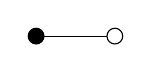
\begin{tikzpicture}
    \draw (0,0) -- (1,0);
    \filldraw[fill=black] (0,0) circle (0.1);
    \filldraw[fill=white] (1,0) circle (0.1);
  \end{tikzpicture}
\end{center}

\begin{center}
  \begin{tabular}{c|c|c|}
    \multicolumn{1}{c}{} &
    \multicolumn{1}{c}{$\selfDef$} &
    \multicolumn{1}{c}{$\nselfDef$} \\ 
    \cline{2-3}
    $\tieNeu$ &
    
    \begin{tikzpicture}
      \draw[fill=white,white] (-1, -1) rectangle (2, 1);
      \draw (0,0) -- (1,0);
      \filldraw[fill=gray] (0,0) circle (0.1);
      \filldraw[fill=gray] (1,0) circle (0.1);
    \end{tikzpicture} &

    \begin{tikzpicture}
      \draw[fill=white,white] (-1, -1) rectangle (2, 1);
      \draw (0,0) -- (1,0);
      \filldraw[fill=white] (0,0) circle (0.1);
      \filldraw[fill=black] (1,0) circle (0.1);
    \end{tikzpicture} \\

    \cline{2-3}
    $\ntieNeu$ &

    \begin{tikzpicture}
      \draw[fill=white,white] (-1, -1) rectangle (2, 1);
      \draw (0,0) -- (1,0);
      \filldraw[fill=black] (0,0) circle (0.1);
      \filldraw[fill=white] (1,0) circle (0.1);
    \end{tikzpicture} &

    \begin{tikzpicture}
      \draw[fill=white,white] (-1, -1) rectangle (2, 1);
      \draw (0,0) -- (1,0);
      \filldraw[fill=white] (0,0) circle (0.1);
      \filldraw[fill=black] (1,0) circle (0.1);
    \end{tikzpicture} \\

    \cline{2-3}
  \end{tabular}
\end{center}

%%%%%%%%%%%%%%%%%%%%%%%%%%%%%%%%%%%%%%%%%%%%%%%%%%%%%%%%%%%%%%%%%%%%%%%%%%%
\section{Notation}
%%%%%%%%%%%%%%%%%%%%%%%%%%%%%%%%%%%%%%%%%%%%%%%%%%%%%%%%%%%%%%%%%%%%%%%%%%%

%%%%%%%%%%%%%%%%%%%%%%%%%%%%%%%%%%%%%%%%%%%%%%%%%%%%%%%%%%%%%%%%%%%%%%%%%%%
\bibliographystyle{unsrt}
\bibliography{bibliography}
%%%%%%%%%%%%%%%%%%%%%%%%%%%%%%%%%%%%%%%%%%%%%%%%%%%%%%%%%%%%%%%%%%%%%%%%%%%

%%%%%%%%%%%%%%%%%%%%%%%%%%%%%%%%%%%%%%%%%%%%%%%%%%%%%%%%%%%%%%%%%%%%%%%%%%%
\end{document}
%%%%%%%%%%%%%%%%%%%%%%%%%%%%%%%%%%%%%%%%%%%%%%%%%%%%%%%%%%%%%%%%%%%%%%%%%%%
